\documentclass[11pt,a4paper]{article}
\usepackage[utf8]{inputenc}
\usepackage{amsmath}
\usepackage{amsfonts}
\usepackage{amssymb}
\usepackage{graphicx}
\author{Ben Augarten, Richard Hwang, Max Johnson}
\title{CS 189: HW5 Report}
\begin{document}
\maketitle
\section{Features Implemented}
\begin{itemize}
\item Decision Trees
\begin{itemize}
\item Impurity Function: Entropy
\item Impurity Function: Gina
\item Impurity Function: Misclassification
\item Stopping Criteria: Number of Points
\item Stopping Criteria: Impurity Reduction
\end{itemize}
\item Random Forest
\begin{itemize}
\item Random selection of features
\item Random selection from K best split points
\end{itemize}
\item Boosted Trees (AdaBoost)
\end{itemize}
\section{Results}
\subsection{Decision Trees}
We implemented Decision Trees with 2 different stopping criteria: Stopping based on the number of points, and stopping based on the reduction of impurity. We also implemented three different impurity functions; Entropy, Gina Impurity, and Misclassification.

Entropy, fully grown: 0.0788\\
Entropy, with leaves of at least 26 nodes: 0.0755\\
Entropy, error vs n nodes:\\
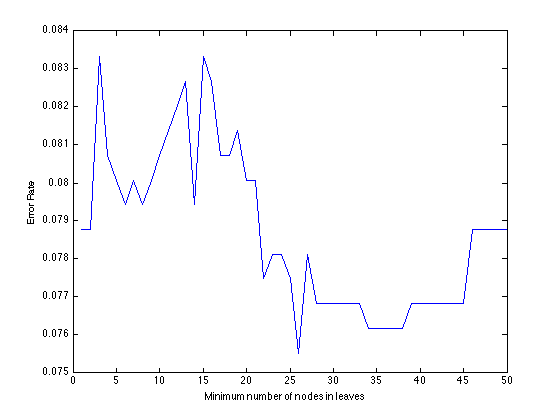
\includegraphics[width=\textwidth]{decision_tree_entropy_error_vs_n_nodes.png}
Variance, fully grown: 0.0872 \\
Variance, with leaves of at least 7 nodes: 0.0846 \\
Variance, error vs n nodes:\\
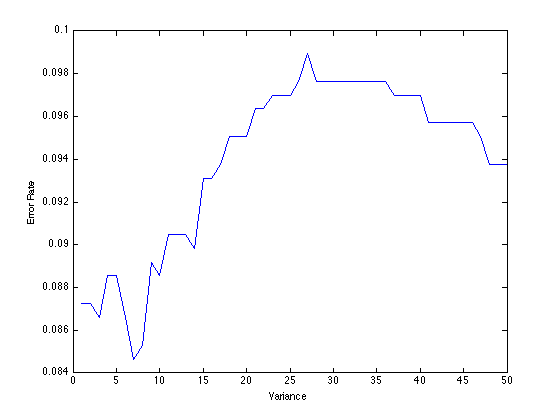
\includegraphics[width=\textwidth]{decision_tree_variance_error_vs_n_nodes.png}
Misclassification, fully grown: 0.0840\\
Misclassification, with leaves of at least 6-11 nodes: 0.0814 \\
Misclassification, error vs n nodes:\\
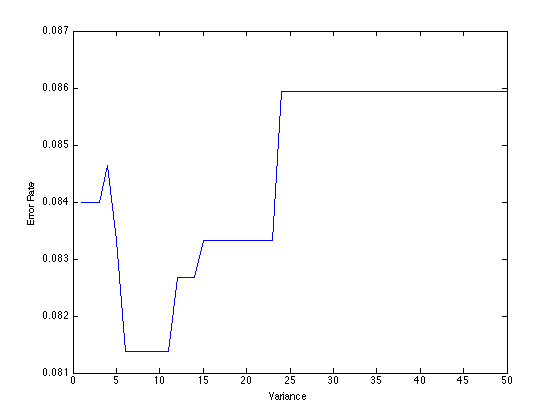
\includegraphics[width=\textwidth]{decision_tree_misclassification_error_vs_n_nodes.png}

\subsection{Random Forests}
Random Feature Selection
Random selection from top-k split points

\subsection{Boosted Trees}
Best error rate: 

\section{References}

\end{document}